%% 
%% Copyright 2026 Elsevier Ltd
%% 
%% This file is part of the 'Elsarticle Bundle'.
%% ---------------------------------------------
%% 
%% It may be distributed under the conditions of the LaTeX Project Public
%% License, either version 1.2 of this license or (at your option) any
%% later version.  The latest version of this license is in
%%    http://www.latex-project.org/lppl.txt
%% and version 1.2 or later is part of all distributions of LaTeX
%% version 1999/12/01 or later.
%% 

\documentclass[preprint,12pt, a4paper]{elsarticle}

\usepackage{amssymb}
\usepackage{hyperref}
\usepackage{xurl}
\usepackage{graphicx}
\setlength{\parindent}{0pt}

\journal{SoftwareX}

\begin{document}
\renewcommand{\labelenumii}{\arabic{enumi}.\arabic{enumii}}

\begin{frontmatter}

\title{PyPIGuard: A Lightweight, Explainable Machine Learning Tool for Pre-Install Detection of Malicious PyPI Packages}

\author{Rahat Ahmed}
\address{Department of Computer Science and Engineering, BRAC University, Dhaka, Bangladesh}

\begin{abstract}
Open-source package registries such as PyPI are increasingly targeted by attackers, yet a benchmark study of deployed detection tools reports false-positive rates between 15\% and 97\%, well above the near-zero tolerance PyPI maintainers require for automated adoption [6]. PyPIGuard is an open-source, deployable tool that classifies PyPI packages as malicious or benign using only static code, Abstract Syntax Tree (AST), and bytecode-level structural features -- without relying on a large language model (LLM) or executing the package. It is deployed as a live web application with a real-time scanner, a file-upload scanner, and a Jupyter notebook malware-import scanner. Trained on 9,723 real packages -- the entire available malicious archive plus freshly-sampled benign packages -- it achieves 0.9993 ROC-AUC and a 0.95 precision / 0.99 recall on the malicious class on independent held-out data, with a median model-inference time of 0.18 ms per package, remaining robust under adversarial evasion and temporal-generalization testing.
\end{abstract}

\begin{keyword}
malware detection \sep software supply chain security \sep machine learning \sep static code analysis \sep PyPI \sep explainable AI
\end{keyword}

\end{frontmatter}

\section*{Required Metadata}
\label{}

\section*{Current code version}
\label{}

\begin{table}[htbp]
\begin{tabular}{|l|p{6.5cm}|p{6.5cm}|}
\hline
\textbf{Nr.} & \textbf{Code metadata description} & \textbf{Please fill in this column} \\
\hline
C1 & Current code version & v1.0 \\
\hline
C2 & Permanent GitHub link to code/repository used for this code version & \url{https://github.com/rahat239/PyPIguard-Research} \\
\hline
C3 & Legal Code License   & MIT License \\
\hline
C4 & Code versioning system used & git \\
\hline
C5 & Software code languages, tools, and services used & Python 3.12, scikit-learn, Flask, HTML/CSS/JavaScript \\
\hline
C6 & Compilation requirements, operating environments \& dependencies & Python $\geq$3.10; \texttt{pip install -r requirements.txt} (pandas, numpy, scikit-learn, joblib, requests, flask, shap); no OS-specific dependencies \\
\hline
C7 & If available Link to developer documentation/manual & \texttt{README.md} in the code repository (C2) \\
\hline
C8 & Support email for questions & rahatahmed537@gmail.com \\
\hline
\end{tabular}
\caption{Code metadata (mandatory)}
\label{tab:metadata}
\end{table}

\textbf{Main text}\\

\begin{enumerate}

\item Motivation and significance

Open-source package registries such as PyPI are foundational to modern software development, but they are increasingly targeted by attackers who publish malicious packages -- often through typosquatting popular libraries such as \texttt{beautifulsoup4}, \texttt{matplotlib}, and \texttt{requests}. In the real \texttt{event-stream} incident (2018) [2], an attacker was granted maintainer access to a popular package simply by offering to help maintain it, and the compromised package reached over 1,600 downstream projects before discovery.

Existing approaches sit at two extremes, leaving a gap PyPIGuard targets. Lightweight metadata-only classifiers are fast but easily gamed once attackers adapt. Heavyweight behavioral models -- e.g., Cerebro [3], requiring 14--25 hours of training and reporting an 81.5\% false-positive rate on PyPI in its own evaluation -- are too slow or imprecise for real-time, pre-install scanning. Vu et al.'s benchmark [6] found 15--97\% false-positive rates across deployed PyPI scanners, and reports administrators consider rates above $\sim$0.01\% operationally unacceptable given daily release volume.

\textbf{The gap PyPIGuard addresses:} a static-analysis classifier simultaneously fast enough for real-time use, explainable per-prediction, and validated against adversarial evasion, temporal drift, and cross-ecosystem transfer -- none jointly reported for the tools in [6]. It is built on the dataset released with [1] and PyPI's official index.

In practical terms: a developer supplies a package name, archive, or notebook; PyPIGuard analyzes it without executing it and returns a CLEARED/FLAGGED verdict, a confidence score, and the specific patterns that drove the decision.

\item Software description

\begin{enumerate}
    \item \textbf{Software architecture.} Figure~\ref{fig:architecture} shows the end-to-end pipeline. A submitted package is first checked against a \textbf{verified-lookup table} of 5,900 packages with ground-truth labels; if found, an instant dataset-backed verdict is returned, visually marked ``verified'' rather than model-predicted. Otherwise, three sequential stages run: (1) a \textbf{feature-extraction layer} retrieves the source (or accepts a local upload) and computes 35 static features via regex, Python's \texttt{ast} module, and \texttt{compile()}-based bytecode inspection, none requiring execution; (2) a \textbf{classification layer} -- a single Random Forest classifier -- outputs a prediction and confidence score; (3) a \textbf{delivery layer} (Flask) formats the verdict with a SHAP [8] explanation and flagged patterns. An \textbf{out-of-distribution safety gate} between (2) and (3) flags verdicts as unreliable when a package's size falls far outside the training range, a behavior added after deployment testing (Section 4).

\begin{figure}[htbp]
\centering
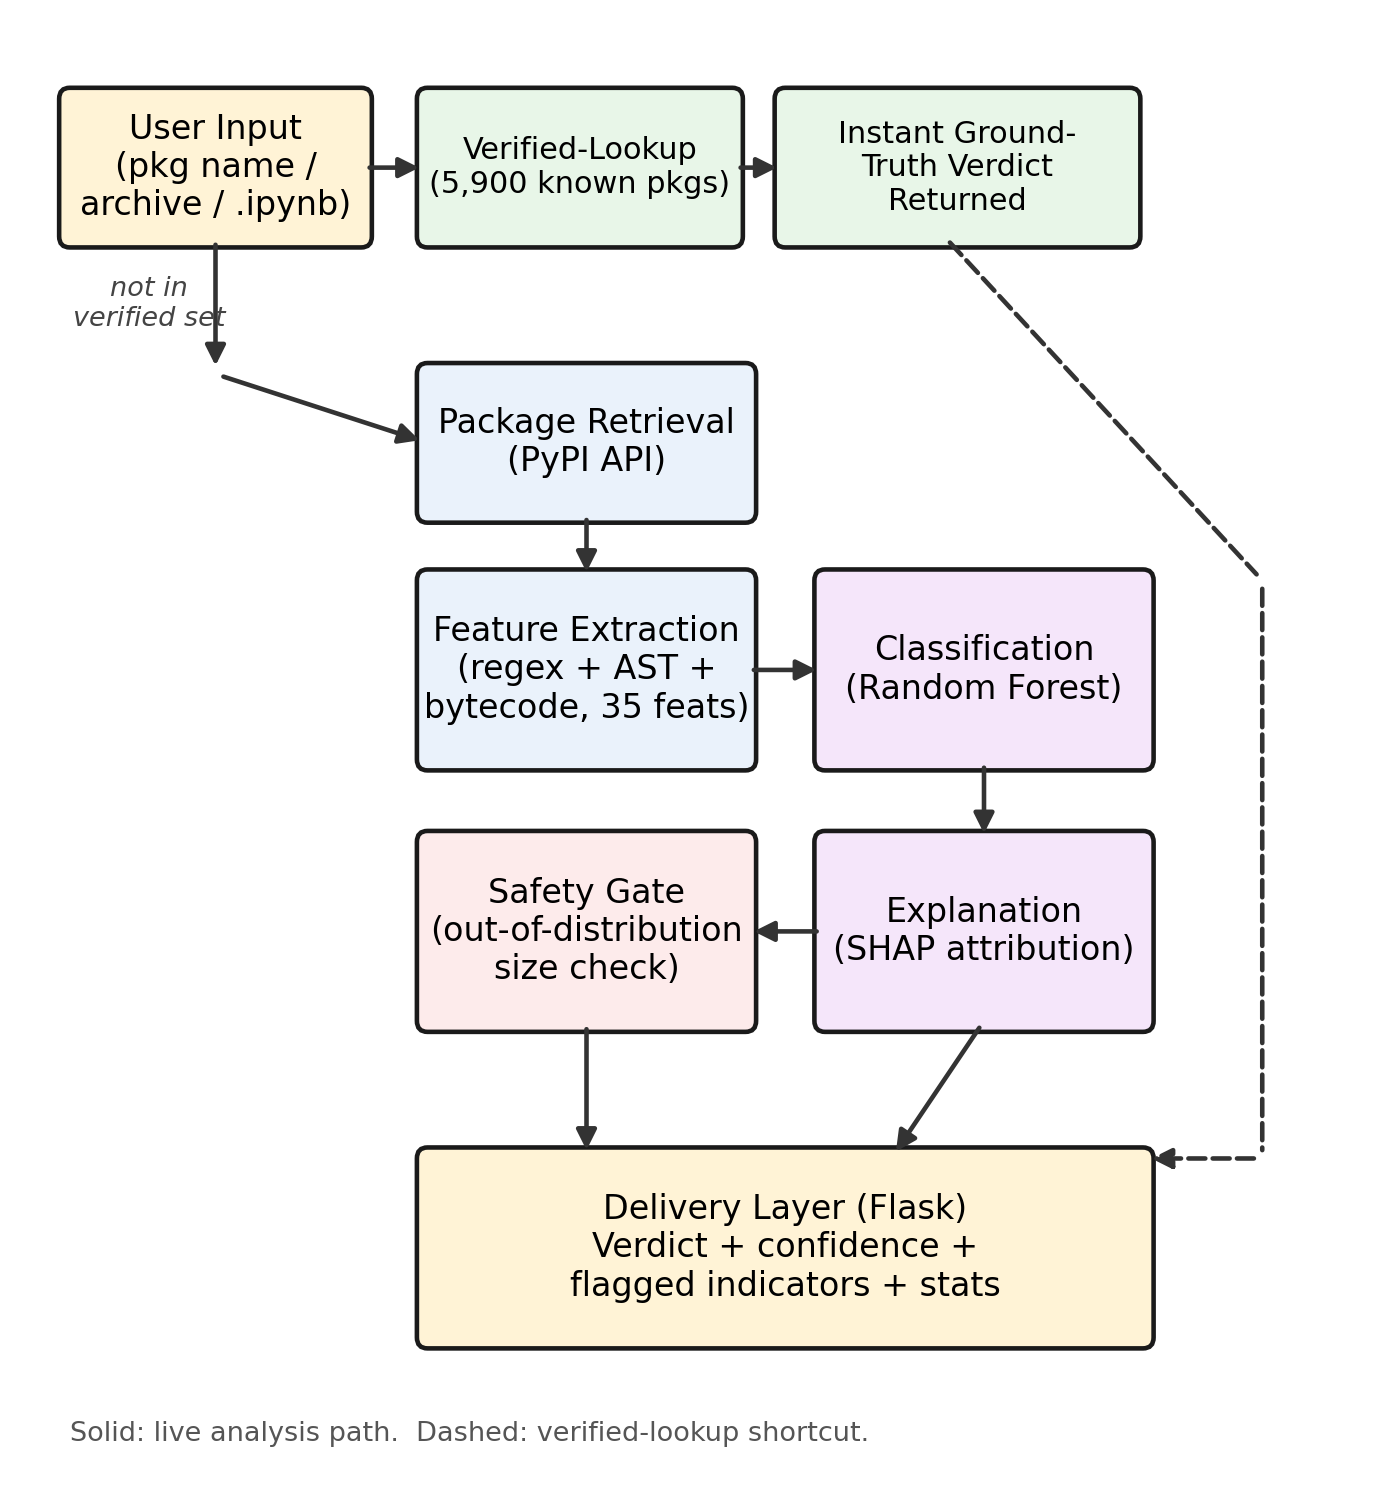
\includegraphics[width=4.5in]{architecture_diagram_v3.png}
\caption{PyPIGuard architecture. Solid arrows: live analysis path. Dashed arrow: verified-lookup shortcut.}
\label{fig:architecture}
\end{figure}

    \item \textbf{Software functionalities.} Three input modes share one verdict format. \textit{Package-name scanning} downloads and analyzes a package live via PyPI's API. \textit{Archive-file scanning} accepts a local \texttt{.tar.gz}/\texttt{.zip}/\texttt{.whl} directly -- useful for historical malware PyPI has since removed. Extraction is hardened against path-traversal (``zip-slip'') attacks, validated against a crafted adversarial archive. \textit{Notebook scanning} parses every \texttt{.ipynb} code cell, extracts \texttt{import}/\texttt{pip install} references, excludes Python's $\sim$300 standard-library modules, resolves import-to-distribution mismatches (e.g., \texttt{cv2}$\to$\texttt{opencv-python}), and reports how many referenced packages are known or suspected malware before execution. Every verdict includes a CLEARED/FLAGGED label, confidence, flagged patterns (e.g., \texttt{eval()} usage, \texttt{setup.py} \texttt{cmdclass} hooks, high-entropy blobs), and a bytecode-level detector for calls like \texttt{getattr(\_\_builtins\_\_,...)} that identifies dynamic dangerous-function invocation independent of the string-construction technique used to hide it. Current limitations: no dynamic/execution-based analysis, and reduced reliability for packages structurally far larger than the training data (flagged via the safety gate above).

    \item \textbf{Sample code snippets.} A representative scan:
\begin{verbatim}
import ast_features, regex_features, joblib
feats = {**regex_features.extract(source_dir),
         **ast_features.extract_ast_features(source_dir)}
model = joblib.load("final_integrated_model.joblib")
proba = model.predict_proba([feats])[0]
verdict = "malicious" if proba[1] > 0.5 else "benign"
explanation = shap_explainer(feats)
\end{verbatim}
The web application wraps this pipeline behind the three input modes; full implementation is in the code repository (C2).
\end{enumerate}

\item Illustrative examples

A user submits a package name (e.g., \texttt{requests}) or uploads a local archive through the web interface. Figure~\ref{fig:screenshots}(a) shows the resulting interface for \texttt{requests}: a stamped CLEARED verdict at 54.7\% confidence and the flagged code patterns contributing to it -- the same package and confidence-calibration case discussed in Section 4. Figure~\ref{fig:screenshots}(b) shows the notebook-upload interface alongside a verified-lookup result: a known-malicious package (\texttt{selfcraftint}) instantly flagged at 100\% confidence from the dataset-backed lookup table described in Section 2, together with the interface's stated limitations.

\begin{figure}[htbp]
\centering
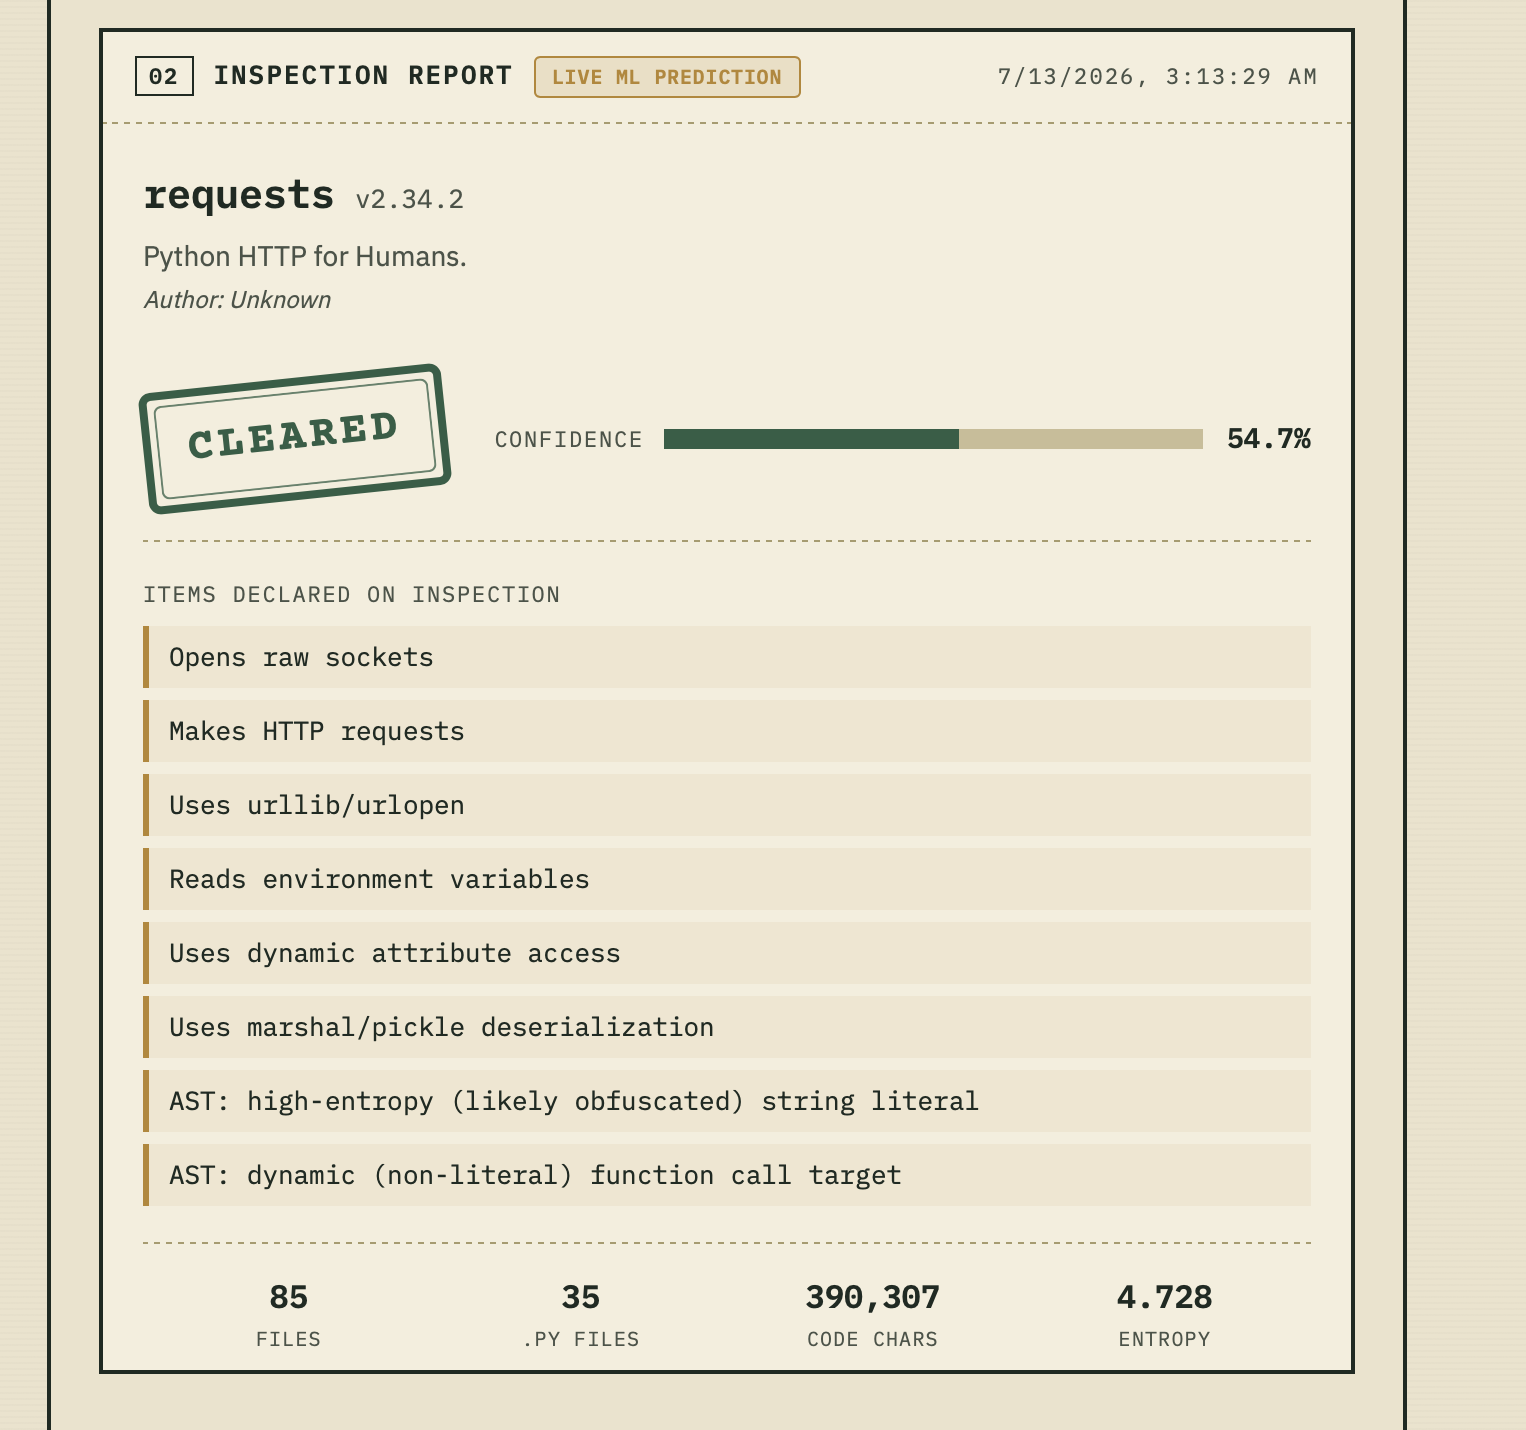
\includegraphics[width=3.4in]{screenshot_scan_result.png}\\[3pt]
\small (a) Package scan result (\texttt{requests})\\[6pt]
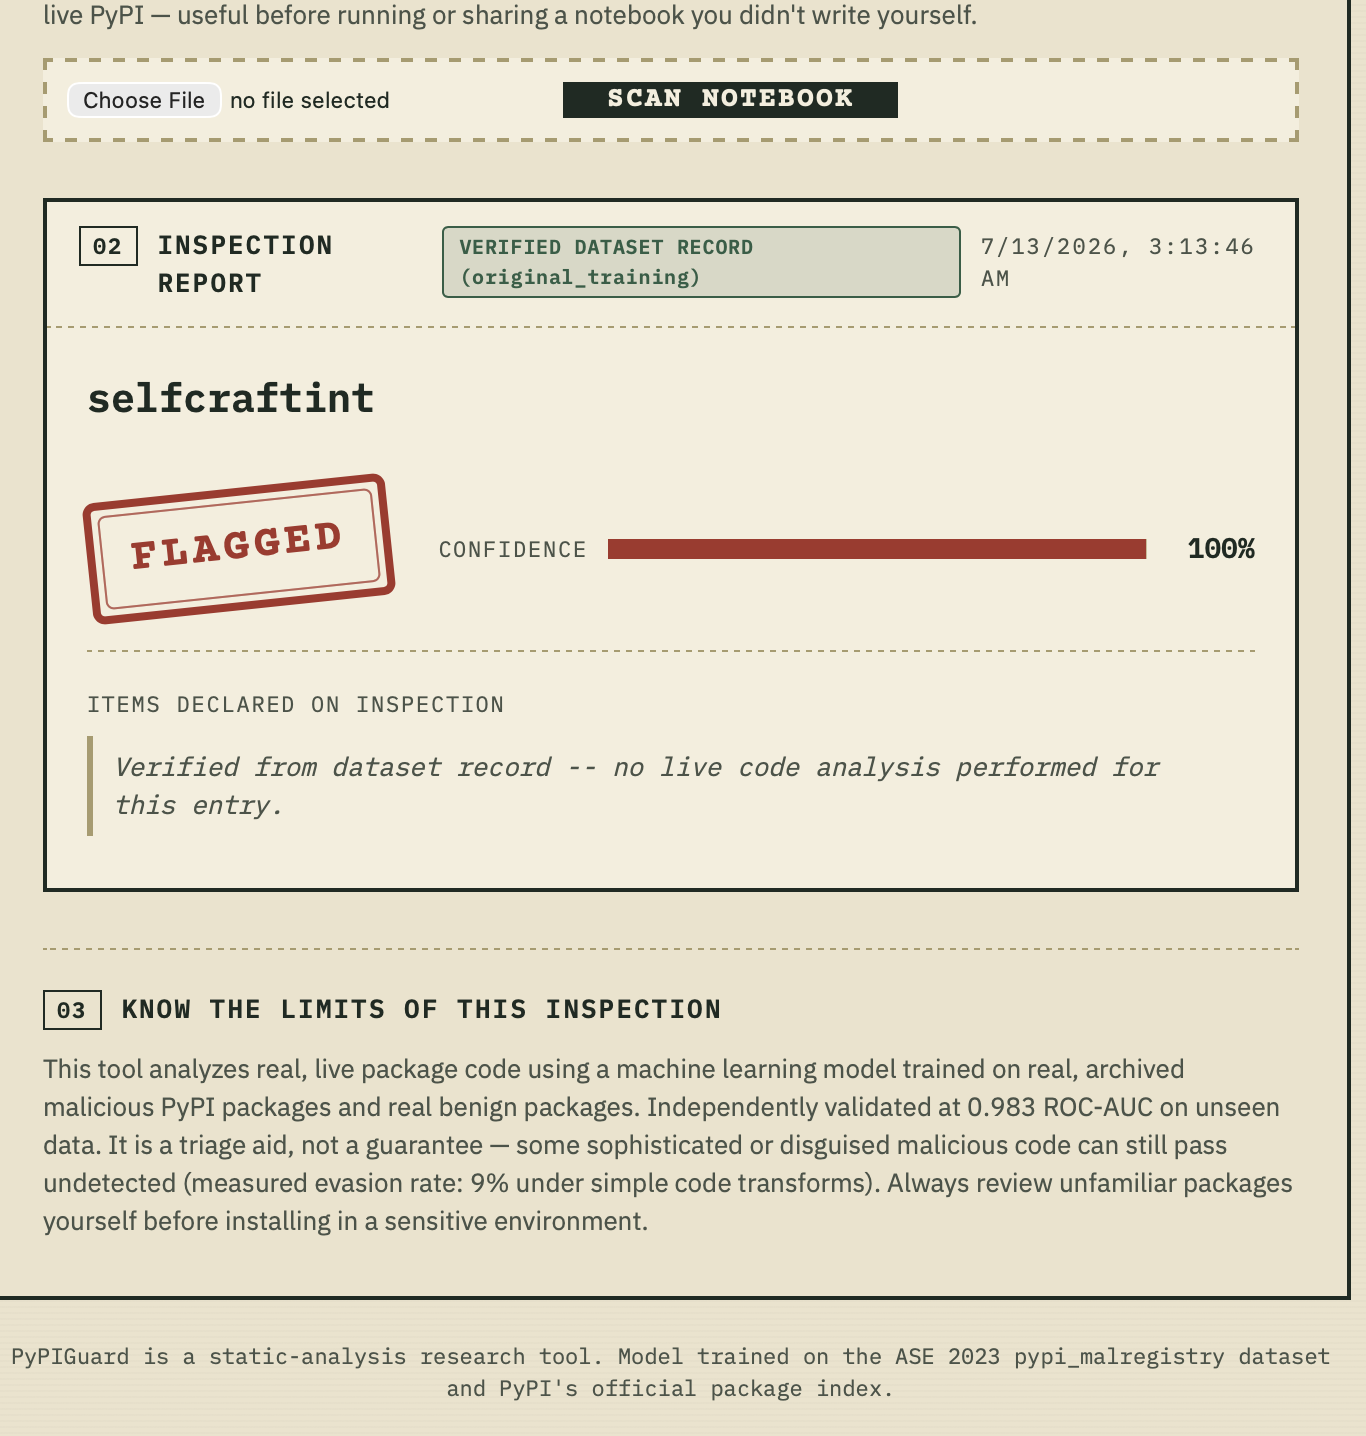
\includegraphics[width=3.4in]{screenshot_notebook_result.png}\\[3pt]
\small (b) Notebook upload \& verified-lookup result
\caption{PyPIGuard web interface: (a) live scan of \texttt{requests}, showing the CLEARED verdict, confidence score, and flagged patterns discussed in Section 4; (b) notebook-scanning upload widget and a verified-lookup verdict for a known-malicious training-set package.}
\label{fig:screenshots}
\end{figure}

\item Impact

\textbf{Evaluation methodology.} The final model was trained on 9,723 labeled packages (7,960 malicious, 1,763 benign; ``at scale'' refers to this set, covering the entire available archive from [1], a $\sim$3.9$\times$ increase over an earlier 2,500-sample version) and validated using 5-fold \textbf{GroupKFold} cross-validation, with an independent 400-package held-out set reported here (zero package-name overlap, verified programmatically). Groups were defined by typosquat family rather than by individual package: malicious samples that are near-duplicate variants of the same base package (e.g., dozens of typosquats of \texttt{requests}) are grouped together so near-duplicates never split across train and test, which a naive random or single-package-based split would not prevent. Results: 0.9993 ROC-AUC, 0.9993 PR-AUC, 0.95 precision, 0.99 recall on the malicious class (Figure~\ref{fig:results}a).

\begin{figure}[htbp]
\centering
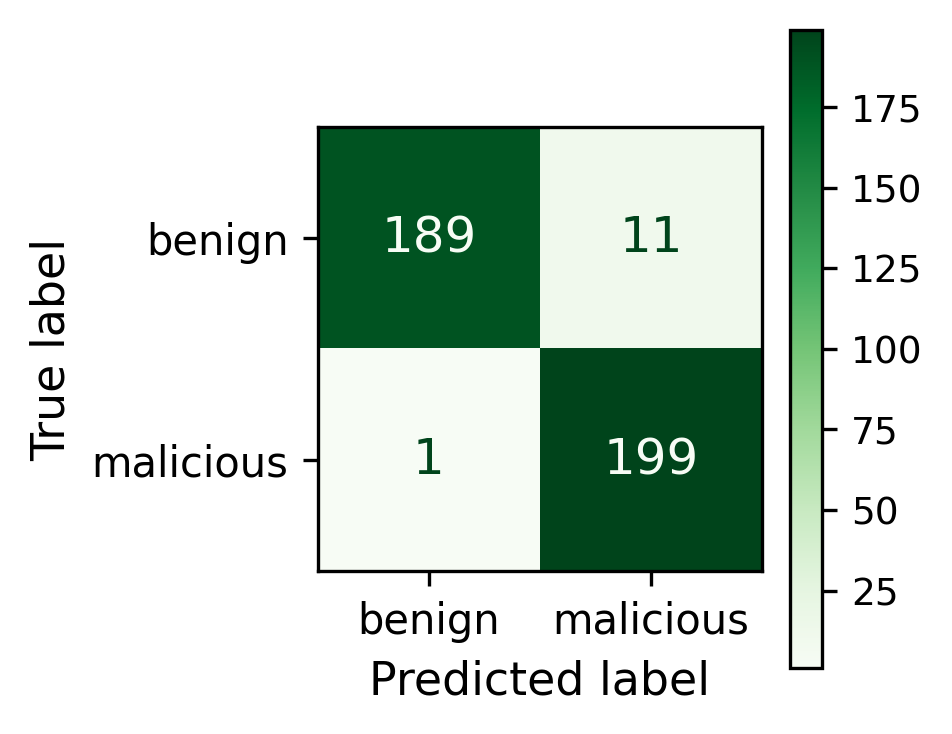
\includegraphics[width=3.17in]{final_integrated_confusion_matrix_v3.png}\\[2pt]
\small (a) Confusion matrix\\[8pt]
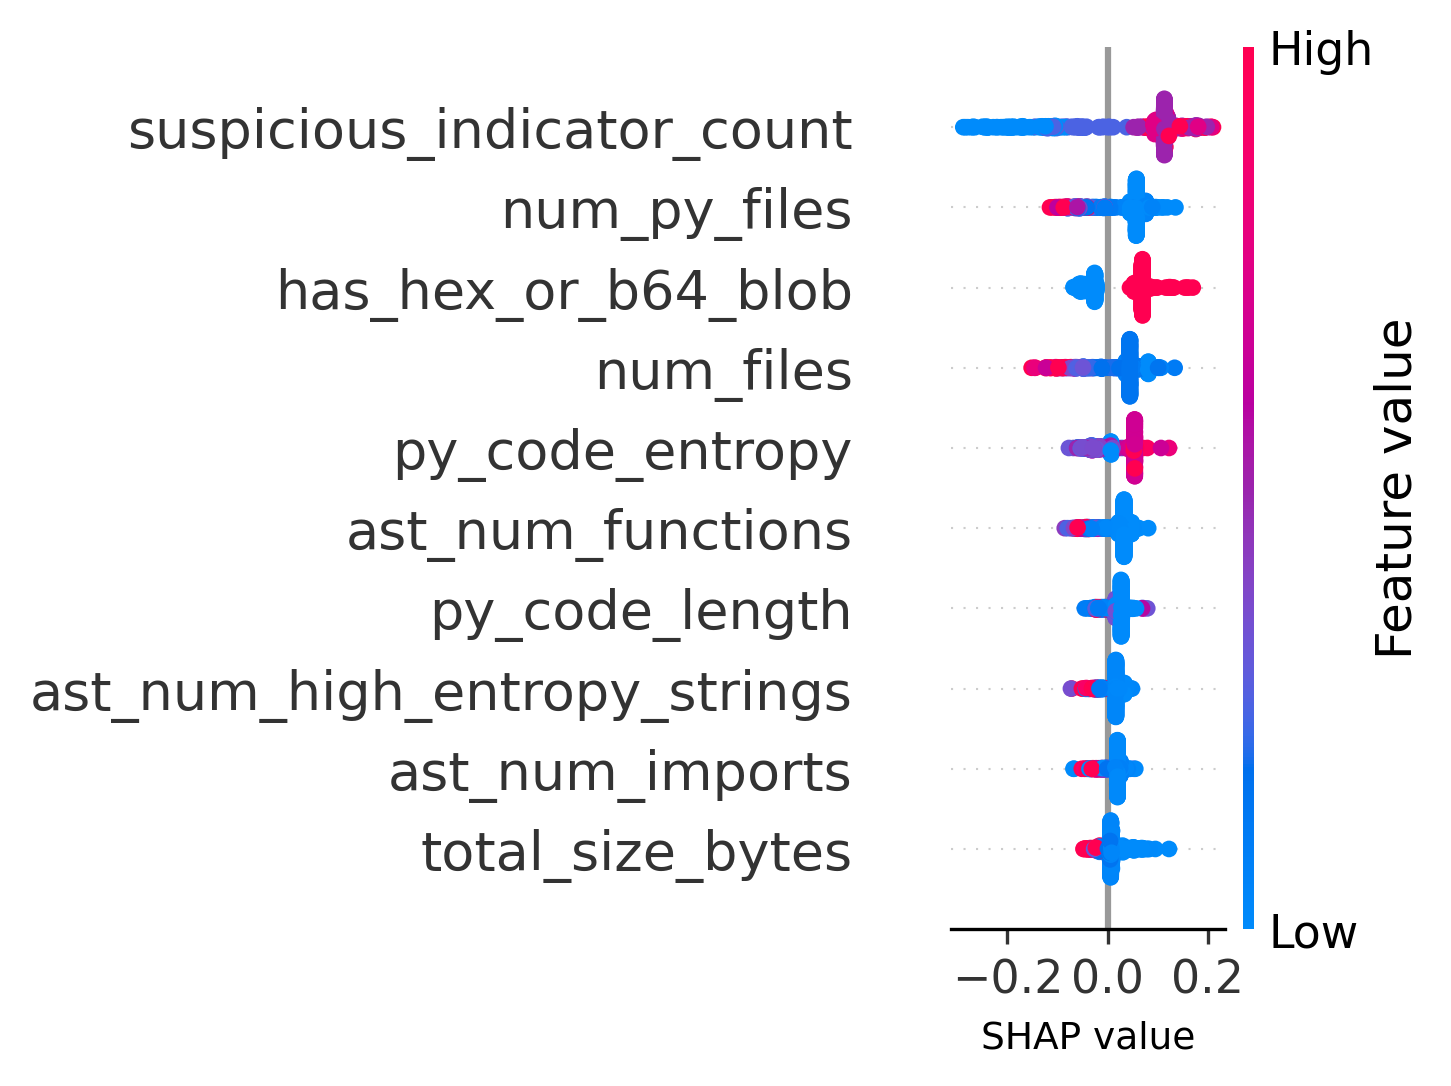
\includegraphics[width=3.4in]{phase4_shap_summary_v4.png}\\[2pt]
\small (b) SHAP summary
\caption{(a) Confusion matrix, held-out set: 189/200 benign correctly cleared (11 FP), 199/200 malicious correctly flagged (1 FN). (b) SHAP global feature importance (top 10 features): horizontal position shows impact on model output, color shows feature value.}
\label{fig:results}
\end{figure}

\textbf{Robustness.} \textit{Temporal}: training only on packages dated before a fixed cutoff and testing exclusively on later packages yields 0.984 ROC-AUC, confirming generalization to malware discovered after training. \textit{Adversarial evasion}: 100 detected malicious packages were paired with behavior-preserving disguises -- e.g., rewriting a direct \texttt{eval(x)} call as an equivalent \texttt{getattr}-based indirection that evades a literal string match. The \textbf{susceptibility gap} -- the fraction of these that evade re-detection -- fell from 9\% (regex-only) to 2\% (AST + bytecode features), an improvement but not a complete fix, reported as a limitation. \textit{Cross-ecosystem}: applying the PyPI-trained model unretrained to real npm packages gives 0.818 ROC-AUC (vs.\ 0.999 in-ecosystem), confirmed consistent at both 2,500- and 9,723-sample scales (0.815 vs.\ 0.818, hence ``across two dataset scales''); recall drops to 0.54, so PyPIGuard should not be deployed on npm without retraining.

For context, Cerebro [3] reports an 81.5\% false-positive rate on PyPI in its own evaluation; PyPIGuard's held-out false-positive rate is 5.5\%. MalGuard [4] reports 91.0\% precision and 94.0\% recall in its own evaluation (independently reproduced by a third-party comparison study); PyPIGuard's held-out precision and recall (95\%, 99\%) exceed both figures. Neither comparison is head-to-head on identical data -- both baselines use their own evaluation datasets -- but together they indicate PyPIGuard operates in a substantially different, more conservative operating regime than either representative baseline.

\textbf{Explainability.} Figure~\ref{fig:results}b shows SHAP global feature importance for the top 10 features. \texttt{suspicious\_indicator\_count} (the aggregate count of triggered regex-based patterns) is the single most influential feature, followed by \texttt{num\_py\_files}, \texttt{has\_hex\_or\_b64\_blob}, and \texttt{num\_files}: packages triggering more suspicious patterns simultaneously, or containing fewer Python files overall, are pushed toward malicious, consistent with thin, single-purpose typosquats; larger file counts push toward benign, consistent with legitimate packages carrying more supporting files (tests, documentation, packaging metadata) than minimal payloads. This is also the feature-interaction mechanism underlying the version-stability finding above: vendored third-party code inflates \texttt{suspicious\_indicator\_count} independent of a package's own behavior.

\textbf{Latency (deployment-testing finding).} We distinguish three previously conflated measures: \textit{model inference} (0.18~ms median), \textit{feature extraction} (0.2--1~ms), and \textit{end-to-end scanning} (PyPI network round-trip plus hosting overhead). A reviewer-observed $\sim$20s scan of \texttt{requests} is attributable entirely to download time and free-tier hosting cold-start, not model inference, which stays sub-millisecond; this is now stated as an explicit deployment limitation.

\textbf{Confidence calibration (deployment-testing finding).} \texttt{requests} was classified benign at 54.3\% confidence during reviewer testing (54.7\% on our own re-verification of the same version, confirming stability across repeated scans) -- correct, but near the decision boundary. Random Forest probability estimates are not calibrated probabilities: bagging averages predictions across trees with high individual variance, which is established to bias ensemble predictions away from the extremes (near 0 or 1) toward the middle of the range [7], independent of any single input's characteristics. We additionally tested version stability directly: scanning five real \texttt{requests} releases spanning 2011--2026 (v0.2.0, v0.9.2, v2.2.0, v2.17.0, v2.34.2) found 3 of 5 \textbf{misclassified as malicious}, one (v2.17.0) at 93.7\% confidence. Investigating the cause, we found these releases bundle vendored copies of their own dependencies (e.g., urllib3, chardet) directly in the source tree, an older packaging convention; this vendored third-party code triggers multiple suspicious-pattern features cumulatively (including a genuine match on our \texttt{getattr} obfuscation detector in v2.2.0's vendored code), inflating the aggregate suspicious-indicator count regardless of \texttt{requests}' own code. This reveals a genuine construct-validity limitation, not merely a confidence-calibration nuance: PyPIGuard's current static features cannot distinguish a package's own suspicious behavior from suspicious patterns present in legitimately vendored third-party code, and this is reported here as an identified limitation rather than a solved problem. The current version (v2.34.2, no longer vendoring dependencies) and one older version (v0.9.2) are both classified correctly; the size-based explanation offered for the single-version case above (85 files/390,307 characters vs.\ a training median of 16/19,431) remains a contributing but not sole factor. A path-traversal (``zip-slip'') vulnerability, found and patched via a crafted adversarial test archive prior to deployment, is documented here for the same transparency reason.

\textbf{Practical impact.} Intended users are developers, students, and CI/CD pre-install gates deciding whether to install a dependency. A false negative risks installing malware; a false positive costs a manual review. Given the 5.5\% FP / 0.5\% FN rates and explicit uncertainty flagging, PyPIGuard is a decision-support triage tool, not an autonomous blocker. It is deployed as a public, live tool (Section 5), testable against real historical malware no longer on the live registry, since PyPI removes malicious packages once discovered.

\textbf{Future work} includes extending static learning to other ecosystems beyond the partial PyPI-to-npm transfer above, and combining PyPIGuard's tabular features with sequence-order information -- a separate matched comparison found a simplified Cerebro-inspired [3] sequence proxy modestly outperforming PyPIGuard (0.983 vs.\ 0.967 ROC-AUC), suggesting sequence information carries signal the flat feature vector misses.

\item Conclusions

PyPIGuard is an open-source, deployed, explainable tool for pre-install detection of malicious PyPI packages, validated through temporal, cross-ecosystem, and adversarial-evasion testing not typically reported together for tools of this scope. It shows that a static, LLM-free analysis approach operates in a substantially different false-positive regime than a benchmarked deep-learning baseline [3], while transparently reporting its boundaries: cross-ecosystem transfer is only partial, adversarial evasion is reduced but not eliminated, static analysis alone leaves dynamic/behavioral attack surfaces uncovered pending access to properly isolated execution infrastructure, and the current free-tier deployment does not represent production-grade latency despite sub-millisecond model inference.

\end{enumerate}

\section*{Acknowledgements}
\label{}

The author thanks the maintainers of the \texttt{pypi\_malregistry} dataset [1] and the Datadog Security Labs malicious-software-packages dataset [5], both of which made this work possible.

\section*{Declaration of Generative AI and AI-assisted technologies in the writing process}
\label{}

During the preparation of this work, the author used ChatGPT (OpenAI) to assist with drafting and restructuring portions of the manuscript, correcting grammatical errors, and refining writing style. After using this tool, the author reviewed, edited, and verified all content for technical accuracy and takes full responsibility for the content of the published article.

\begin{thebibliography}{00}

\bibitem{malregistry} W. Guo, Z. Xu, C. Liu, C. Huang, Y. Fang, Y. Liu, An Empirical Study of Malicious Code In PyPI Ecosystem, in: Proceedings of the 38th IEEE/ACM International Conference on Automated Software Engineering (ASE), IEEE, 2023, pp. 166--177.
\bibitem{backstabber} M. Ohm, H. Plate, A. Sykosch, M. Meier, Backstabber's Knife Collection: A Review of Open Source Software Supply Chain Attacks, DIMVA, 2020.
\bibitem{cerebro} J. Zhang, K. Huang, B. Chen, C. Wang, Z. Tian, X. Peng, Killing Two Birds with One Stone: Malicious Package Detection in NPM and PyPI Using a Single Model of Malicious Behavior Sequence, ACM Transactions on Software Engineering and Methodology, 2025.
\bibitem{malguard} X. Gao et al., MalGuard: Towards Real-Time, Accurate, and Actionable Detection of Malicious Packages in PyPI Ecosystem, USENIX Security, 2025.
\bibitem{datadog} Malicious Software Packages Dataset, Datadog Security Labs, 2023.
\bibitem{wyss} D.-L. Vu, Z. Newman, J.S. Meyers, A Benchmark Comparison of Python Malware Detection Approaches, arXiv:2209.13288, 2022.
\bibitem{calibration} A. Niculescu-Mizil, R. Caruana, Predicting Good Probabilities With Supervised Learning, in: Proceedings of the 22nd International Conference on Machine Learning (ICML), 2005, pp. 625--632.
\bibitem{shap} S.M. Lundberg, S.-I. Lee, A Unified Approach to Interpreting Model Predictions, in: Advances in Neural Information Processing Systems 30 (NeurIPS), 2017, pp. 4765--4774.

\end{thebibliography}

\section*{Current executable software version}
\label{}

Live demonstration available at: \url{https://rahat239.github.io/Malware-classifier/}

\end{document}
\endinput